\section{Harrison Armory Tokugawa}

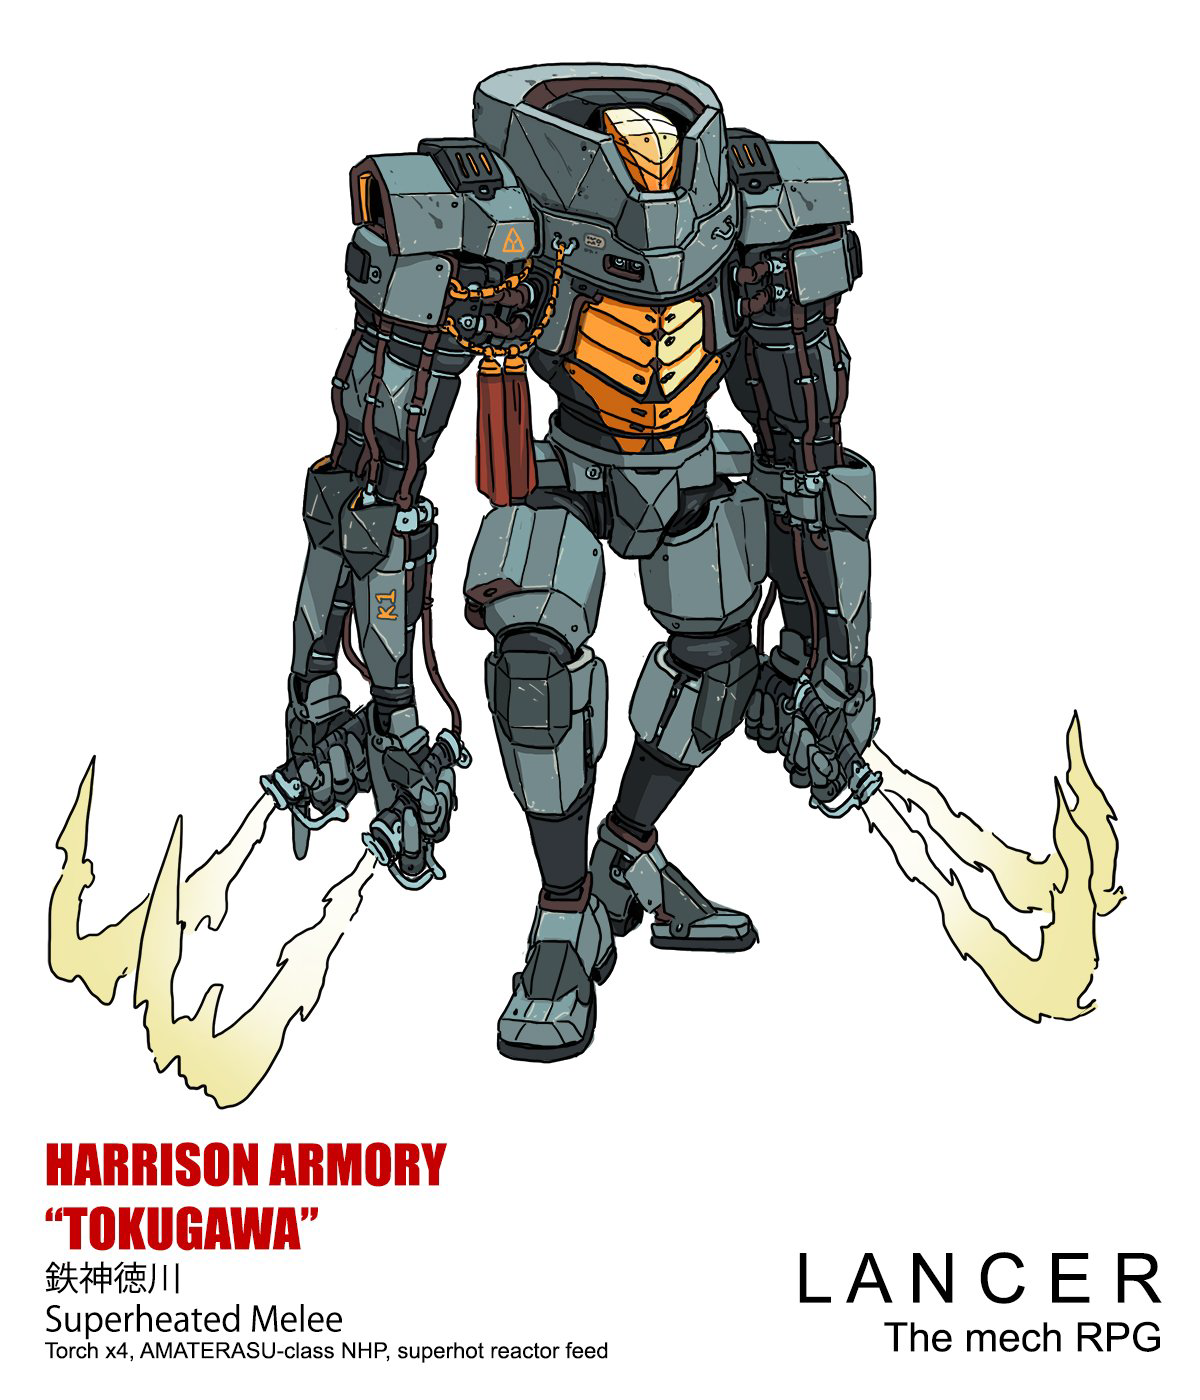
\includegraphics{Tokugawa}

                             HARRISON ARMORY TOKUGAWA

HA’s TOKUGAWA chassis is a relative newcomer on the market, popular in core systems for security and

CQB/ breach applications. The TOKUGAWA is a large, imposing mech, a sturdy platform from which the
recommended kit can draw the necessary power it needs in order to perform within optimum parameters.

                                                  License:
I. External batteries, Annihilator

II. TOKUGAWA FRAME, Experimental heat sink, Plasma Lash

III. Torch, AMATERASU class NHP





                                                    TOKUGAWA

  HP: 8            Evasion: 8                              Speed: 4             Heat Cap: 8         Sensors: 10

  Armor: 1         E-Defense: 6                            Size: 1              Repair Cap: 4       Tech Attack: -1

                                                        TRAITS:

  Reactor Flare: The Tokugawa’s energy weapon attacks deal +1d6 bonus damage if it has 2 or less
  reactor stress remaining

  Plasma Sheathe: While the Tokugawa is in the danger zone, it’s energy weapon attacks deal all bonus
  damage as Burn

                                                 SYSTEM POINTS: 6

                                                       MOUNTS:

  Flexible Mount                       Main Mount                               Main Mount

                                                    CORE system

                                             Superheated Reactor Feed

  A certain breed of pilot rides the very edge of catastrophe, swinging between an equal chance of
  success and failure each moment. Tokugawa pilots are familiar with the howl of their chassis’s heat
  warning, the warbling siren a song of destruction: with a superheated reactor feed, Tok pilots ramp their
  heat debt to the max in order to supercharge their energy weapons. This allows them to churn out
  damage and make no friends in the engineering bay, should they not melt into a ball of slag before they
  make it back from the line.

  Active (requires 1 core power):
  Radiance
  Protocol

  Choose 1 energy weapon your mech is wielding. If it is a ranged weapon, its range increases by 5, if it
  is a melee weapon, its threat increases by +1. For the rest of this combat, this weapon also deals +1d6
  Burn damage (roll on each attack). However, each time you fire this weapon, you gain +3 heat.

External Batteries
External batteries are by no means a Harrison Armory exclusive, but HA literature will ensure you that HA-

Brand POWERALL cells are the longest lasting, fastest cycling, and highest capacity solid state cells
available. A consequence of their high capacity is a proportionate increase in volatility if the system should
ever be damaged, but pilots looking to utilize HA technology agree through continued use to absolve HA

from all liability.

2 SP, Unique





Your ranged weapons that deal energy damage gain +5 range, and your melee weapons that
deal energy damage gain +1 threat. If you take structure damage, this system explodes and is
destroyed, dealing 3 AP explosive damage to your mech. This damage can’t be prevented in any
way.


Annihilator

HA specializes in conventional and unconventional arms development; solutions to tactical problems are
designed both in the lab and in the field, often the latter outperforming the former in combat situations. The

Annihilator takes its name from pilots’ slang for a field-rigged weapon developed during the Bradbury
Rebellion, when desperate resistance pilots machined a way of shunting the incredible waste heat of their
core’s reactor into a directed blast.

Main CQB

AP, 2 heat (self)

Range 5, Threat 3

1d3+1 energy damage

This weapon creates an energy pulse for burst 1 around its target’s location on successful hit.
Actors caught in the area must pass an engineering check or take 1d3+1 AP energy damage.


Experimental Heat Sink

The Harrison Armory DEEP WELL system is a part of their VANGUARD line of equipment available to
licensed HA beta testers. Though a complicated and delicate weave of heat exchangers, Harrison Armor’s

DEEP WELL system attempts to recycle the heat generated by a chassis’ systems into useable energy.
While the system works well, the delicate nature of the exchange renders the DEEP WELL highly volatile.

4 SP, Unique
While your mech is in the Danger Zone, it has resistance to heat.


Plasma Lash

A threat at multiple ranges, the Lash was designed following the Armory’s review of data collected from the
Hercynian Crisis. After-action reports noted the efficacy of thermal and thermobaric weapons against
hardened targets, but made constant reference to the limitations placed upon conventional thermal

weapons: the need for atmosphere-specific fuel, the impact of prevailing weather conditions, the necessity
of atmosphere.

Enter the Plasma Lash, an early development into plasma weaponry. Firing an excited toroid of plasma, the
Lash can be used as a ranged weapon with a delayed-detonation, or, essentially, a point-blank melee
weapon; if used at point blank range, the toroid is detonated inside of its launcher, directing an intense

thermal blast directly at its target.

Main Melee or Main CQB

2 heat (self)

Range 5, Threat 3

1 Energy Damage + Burn 3





This weapon can be used with either profile, but not both in the same round.


Torch

The Armory’s TORCH is a backbone core weapon: a heavy, two-handed, dual crescent-bladed plasma
torch. The melee weapon is powered by its wielder’s reactor, connected by both powerlines and inert
cabling; it can be separated into two torch-axes, and its plasma blades are capable of being tuned into new

shapes. A common sight in CQB situations, the torch has of late become a status symbol among pilot
officers, many preferring to carry them alongside a smaller auxiliary weapon.

Main Melee

1 heat (self)

Threat 1

1d6 energy damage + Burn 2


AMATERASU-class NHP
AMATERASU came to prominence in the Armory NHP think tank after its repeated victories in war thought-

games. AMATERASU is characterized by its brash, enthusiastic personality, often expressing frustration
with timid pilots who have it in their employ; however, this bombastic personality hides a calculating,

brilliant tactical mind that feeds information to pilots often faster then they can process it. AMATERASU’s
combat doctrine demands action and impetus, a chaotic blend of reckless maneuvering and aggressive
offense that keeps defenders beleaguered and unable to respond with any great efficacy. Pilots willing to

partner with AMATERASU should be aware that this attack style often leaves their cores vulnerable to
counterattack, and that this NHP enjoys what it calls “good-natured ribbing”.

3 SP, Unique
AI
Your mech gains the AI property and the AMATERASU protocol
	        AMATERASU protocol
	        Protocol
	        1d3+3 heat (self)
         Increase the bonus damage on hit of your next ranged or melee attack this turn by your
         current heat after activating this protocol. The chosen weapon must deal at least partly
         energy damage.
